
\chapter{The Lisp interpreter}

\par The size of the MalbolgeLISP interpreter is approximately 350 MB, and it requires a minimum of 1.5 GB of system memory to facilitate optimal usage conditions. The default arithmetic operators work on 26-bit wide integers, which is also MalbolgeLISP's pointer size; this means that the interpreter is capable of addressing around 67 million 26-bit words of memory. It is generally recommended to execute MalbolgeLISP under a fixed rotation width interpreter locked at 19 trits for the best possible performance characteristics without trading functionality.

\par After execution, MalbolgeLISP displays a banner similar to the one below:

\begin{verbatim}
MALBOLGELISP V1.2 (2020-2021, PALAIOLOGOS)
DOT COMMANDS: .F(eatures) .A(uthor) .R(eset) .M(emory) .S(ymbols) .E(xport) .I(mport)
% 
\end{verbatim}

\par The MalbolgeLISP REPL accepts two kinds of data - dot commands and MalbolgeLISP expressions. The following is the feature list reported by the interpreter, consisting of 76 builtin functions:

\begin{verbatim}
% .F
' ~ + - % < > = ! & | * / ^ def defun lambda
cond print atom cons car cdr if let defmacro
iota size nth map filter eval append append'
>= <= max min /= rev any every sort zip id
flatten flatmap tie fold zipwith iterate iterateN
where replicate count take take' drop drop' bind
atop intersperse scan monad dyad selfie commute
fold' scan' uniq off +' -' fork lazy lift bruijn
\end{verbatim}

\section{MalbolgeLISP's memory model and dot commands}

\par MalbolgeLISP's memory is split between the heap and the stack. The stack is located at the end of addressable memory and grows downwards, while the heap grows upwards. The space in the heap is allocated using a bump allocator with support for rewinding. The current memory usage can be checked using the \verb|.M| dot command, as presented below:

\begin{verbatim}
% .M
6W USED
% # some operations follow...
% .M
125W USED
\end{verbatim}

\par Clearing the memory is possible using the \verb|.R| dot command. \verb|.R| resets the bump allocator's internal pointer to the default value, removes \textit{all} objects and clears the global table. A few objects are preallocated on the heap\footnote{strings: \verb|quote|, \verb|lazy|, \verb|x|, \verb|y|; numbers: \verb|1| - true, \verb|0| - false}.

\par It is possible to create a saved interpreter state using the \verb|.E| dot command, which dumps the data pointers (to preallocated data, global table pointer and interned string list), dump size and the resulting data starting from the beginning of the memory to the logical end of used memory, as indicated by the bump allocator's internal pointer. Loading the image is to be performed via the use of the \verb|.I| dot command. The loaded data is not checked for validity, nor is it compacted before exporting or after importing. This procedure can be performed by external software, knowing the format of the memory dump.

\par The following data structures are employed by the MalbolgeLISP interpreter:

\begin{itemize}
    \item An atom, which is a tagged union of all the possible data types. The mappings between type and the tag follow\footnote{When the \verb|atom| function is used, it returns one of the following integers that correspond to a type}:
    \begin{itemize}
        \item 0 - Number
        \item 1 - Unbound atom
        \item 2 - List
        \item 3 - Closure
        \item 4 - Macro
        \item 5 - Partially applied function object produced by \verb|bind|
        \item 6 - Partially applied function object produced by \verb|bind'|\footnote{\verb|((bind f x y) z)| $\Leftrightarrow$ \verb|(f x y z)|, while \verb|((bind' f x y) z)| $\Leftrightarrow$ \verb|(f z x y)|}
        \item 7 - Function composition object produced by \verb|atop|.
        \item 8 - Fork object produced by \verb|fork|.
        \item 9 - NTH object produced by the \verb|#N| syntax.
        \item 10 - Tack object produced by the \verb|$N| syntax.
        \item 11 - Lazily evaluated value.
        \item 12 - Nothing (\textit{NULL}, which is also a valid list)
        \item 13+ - Invalid
    \end{itemize}
    \item An unbound atom, which is a pointer to the first character of an interned string.
    \item The interned string table is a linked list of unbound atoms. It is built at parse time, such that every string atom referenced in the code is placed in the interned string table, which reduces memory usage\footnote{this is because every string at the moment of creation is compared with every existing string within the interned string table. A runtime performance cost is incurred due to this technique to reduce memory usage.}.
    \item A list, which is a pointer to a tuple consisting of the list head, which is an atom, and the list tail, which is the next list node.
    \item A closure is a symbol table tied to the list containing the list of arguments and the list with code.
    \item A symbol table is a pointer to a triplet of the key, which is a pointer to the first character of the string representing the entry, the value, which is an atom, and the pointer to the next symbol table entry.
    \item A macro is a list consisting of the argument list and the code list.
    \item Partially applied function objects of both kinds are the beheaded lists along \verb|bind| and \verb|bind'|.
    \item Function composition objects consist of a beheaded list passed along \verb|atop|.
    \item Fork objects consist of a list of functions produced by beheading the list passed along \verb|fork|.
    \item nth and tack objects are numbers that can be created only during the parse time.
    \item Lazily evaluated values are created using the \verb|lazy| built-in word. Lazily evaluated value is a list with code to which the caller's environment has been bound.
\end{itemize}

\par The exported memory blob starts with the following header:

\begin{itemize}
    \item The pointer to the global table
    \item The pointer to the \verb|quote| atom.
    \item The pointer to the \verb|lazy| atom.
    \item The pointer to the \verb|fork| atom.
    \item The pointer to the \verb|x| atom.
    \item The pointer to the \verb|y| atom.
    \item The pointer to the \verb|1| (truthy value) atom.
    \item The pointer to the \verb|0| (falsy value) atom.
    \item The pointer to the first interned string table entry.
    \item The dump size in words.
\end{itemize}

\par On the transport layer, the exported memory format is a sequence of five byte ASCII representations of the 26-bit values used by the interpreter, where the first four characters each map in total 24 bits, and the last character maps the remaining 2 bits.

\par The data is extracted from the number starting from the back. Then, they are encoded into ASCII values using the following LUT:

\begin{verbatim}
&l_n2a
txt "QWERTYUIOPASDFGHJKLZXCVBNM0123456789!@#$%^&*()_+-=[]cb;':/?.>,<a"
\end{verbatim}

\par The following LUT is used for turning ASCII values minus 33 back to numbers:

\begin{verbatim}
&l_a2n
$(gen_vec({
  36,0,38,39,40,42,55,44,45,43,47,61,48,59,57,
  26,27,28,29,30,31,32,33,34,35,56,54,62,49,60,
  58,37,10,23,21,12,2,13,14,15,7,16,17,18,25,24,
  8,9,0,3,11,4,6,22,1,20,5,19,50,0,51,41,46,0,63,
  53,52}))
\end{verbatim}

\par The symbols that are defined in the global table of the current session are listed using the \verb|.S| dot command, as illustrated below:

\begin{verbatim}
% ; Binding a few variables
% (def succ (monad [x + 1]))
................|..
(lambda (x) (+ x 1))
% (def pred (monad [x - 1]))
................|..
(lambda (x) (- x 1))
% (def numid (atop succ pred))
...........|......
bind/syn
% (def x 5)
.......|..
5
% ; Checking the memory usage and
% ; printing the symbol table.
% .M
199W USED
% .S
x numid pred succ
%
\end{verbatim}

\par The last command the interpreter claims to recognise is .A, shown as follows - although there exists one more undocumented dot command (besides the ones listed in the REPL's banner) that is outside the scope of this document:

\begin{verbatim}
% .A
kamila szewczyk (https://kamila.akagi.moe/), fall 2020 - fall 2021.
\end{verbatim}

\par Unrecognised dot commands cause the interpreter to quit, although the preferred way of quitting the interpreter is \verb|(off)|.

\begin{verbatim}
% .Z
Eh?
\end{verbatim}

\section{Parsing and evaluation overview}

\par The MalbolgeLISP grammar is defined as follows:

\begin{verbatim}
toplevel = atom / dc
dc = "." [A-Z]
atom = _ (null / comment / number / list / quote / lazy / string / nth / tack)
null = "null"
string = [^ \n\[\]\(\)]+
nth = "#" number
tack = "$" number
quote = "'" atom
lazy = "?" atom
list = parlist / sqlist / forklist
parlist = "(" listbody
sqlist = "[" sqlistbody
forklist = "{" forklistbody
listbody = (atom listbody) / ")"
sqlistbody = (atom sqlistbody) / "]"
forklistbody = (atom forklistbody) / "}"
comment = ";" [^\n]+ "\n" atom
number = [0-9]+
_ = [ \n]?
\end{verbatim}

\par \verb|null| is a special construct. It can be used as an empty list with most primitives (like \verb|'()|), and is generally yielded by operations like \verb|cdr| on a single-element list. This grammar describes the input deemed acceptable by the interpreter, which means that it is able to parse dot commands as well as Lisp expressions.

\par Square bracket lists have different semantics from normal lists. Namely, \verb|[a f b c ...]| $\Leftrightarrow$ \verb|(f a b c ...)|\footnote{A feature borrowed from Haskell - \verb|4 `mod` 3| $\Leftrightarrow$ \verb|mod 4 3|}. Conversion between square brace syntax and normal list syntax is performed at parse time and yields no additional run-time performance cost.

\par When an expression is entered, the interpreter begins the parsing stage. Each step of the parsing process is visually represented by a dot printed in the interpreter's output. Upon completion, a pipe is printed to separate the parsing stages from the evaluation stages, and the interpreter begins to print dots for each evaluation step.

\par The evaluation process is bound to the following rules in the given order:

\begin{itemize}
    \item If the input expression proves to be a simple atom, i.e. it is \textit{NULL}, is not a list, or the contents of the list are \textit{NULL}:
    \begin{itemize}
        \item If it is a bounded or unbounded string atom, then it its presence will be checked in the local value table, and then in the global value table.
        \item Otherwise, the atom is returned verbatim.
        \item All of these actions include special handling of lazily evaluated values.
    \end{itemize}
    \item Otherwise, it is considered a list. Based on the type of the list's evaluated head, the following operations are to be performed:
    \begin{itemize}
        \item Closure - create a new table made out of evaluated lambda arguments, append the closure ancestor's symbol table, then evaluate the closure's body.
        \item Bind - clone the already applied argument list, append the current argument list and evaluate the expression. Because of this design, partial application is stackable.
        \item Tack - out of the list containing the tack, pick $n$-th element and evaluate it.
        \item Unbound atom - perform a built-in operation\footnote{like \verb|car|, \verb|scan| or \verb|+|}.
        \item Reverse bind - clone the current argument list and insert it straight after the partially applied function. Then, evaluate the expression.
        \item Macro - create a new table made out of macro arguments (unevaluated) and evaluate the macro's body.
        \item Fork - create a resulting list consisting of just the first function passed to fork, and for each supplied function to the fork except the first one, cons it to the argument list and append it to the resulting list. Then, evaluate the resulting list.
        \item Nth - out of the list supplied as the only argument, pick the $n$-th element and evaluate it.
    \end{itemize}
    \item Lazy values are evaluated when needed by a separate function, which evaluates them as lambda expressions.
\end{itemize}

\par It is not possible to evaluate a list with a non-callable head from within MalbolgeLISP. Consequently, \verb|(uniq (2 3 3))| and any other expressions that make use of unquoted data lists will result in an error. Quoting (via \verb|'(...)| or \verb|(quote ...)|) prevents evaluation, while \verb|eval| forces it.

\subsection{Strict definition of equality}

\par Equality checks within MalbolgeLISP are obedient to the following rules:

\begin{itemize}
    \item If pointers to the atoms are equal, the atoms are compared equal.
    \item If both atoms are \textit{NULL}, the atoms are compared equal.
    \item If the types of both atoms differ, the atoms are compared unequal.
    \item If any of the atoms is a number, their numerical value is compared.
    \item If any of the atoms is unbounded (i.e. a string), they are compared character by character.
    \item If any of the atoms is a list, the list is traversed and the the equality rules are applied on every list element. Only of all list elements compare equal they are compared equal.
    \item Otherwise, the atoms are compared unequal. For this reason\footnote{only in non-trivial cases, i.e. not outlined above} closures, partially applied functions, forks and atops compare unequal.
\end{itemize}

\par Inequality is checked by inverting the result of equality checking. There exists total ordering on numbers, but nothing else\footnote{hence the \verb|sort| function works only with one-deep, numeric lists}.

\subsection{Efficient built-in function recognition}

\par MalbolgeLISP v1.2 employs a novel way of built-in function recognition, which uses hashing to accomplish it's task. Since unbound atoms can be compared and printed, not every string atom can be hashed\footnote{doing so would carry losing entropy as a consequence}. The string atoms are hashed before mathematical operators and other single-character functions are processed\footnote{since i.a. the \verb|gcd| and \verb|lcm| functions are hashed, even though \verb|+| or \verb|-| don't require hashing}. The code follows:

\begin{verbatim}
;      f←3⊥97-⍨⎕ucs
;      f 'iterateN' ⍝ example usage
; 33860

; r1 => the output
; r2 => pointer to the function name
; r3 => trashed
@hash
    clr r1
@hash_loop
    lods r3, r2
    ceq r3, 0
    cret
    mul r1, 3
    sub r3, .a
    add r1, r3
    jmp %hash_loop
\end{verbatim}

\par This hashing algorithm has a somewhat subtle flaw - it's prone to collisions and MalbolgeLISP was unlucky enough to be affected by it:

\begin{verbatim}
      'any' ≡⍥f 'gcd'
1
\end{verbatim}

\par For this reason, the code employs an additional check for the first letter of the string atom if it's hash is equal to 63.

\subsection{List cloning}

\par Since list contents in MalbolgeLISP can't be mutated\footnote{operations like \verb|map| create a new list each time}, they don't have to be cloned often. Consider the following list:

\begin{figure}[H]
\centering
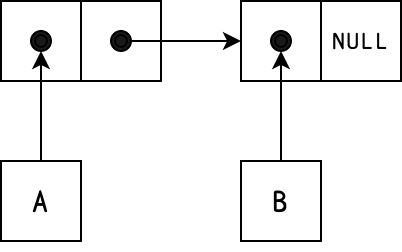
\includegraphics[width=0.3\textwidth]{figures/plist_1.png}
\caption{A flat two-element list consisting of unbound atoms A and B}
\end{figure}

\par The end of the list is marked with \textit{NULL}, to signify that no further nodes are a part of it. Some operations on lists don't require cloning them - for instance, beheading the list (omitting the first element) can be accomplished as taking the tail of the first node in the list - all pointers to the nodes of this list are still valid and point to the desired data:

\begin{figure}[H]
\centering
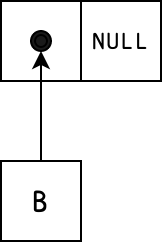
\includegraphics[width=0.1\textwidth]{figures/plist_3.png}
\caption{A beheaded list with only atom B left}
\end{figure}

\par Prepending content to a list (creating a new list node and setting it's tail) can also be done without a copy - \verb|(cons C l)| yields the following result:

\begin{figure}[H]
\centering
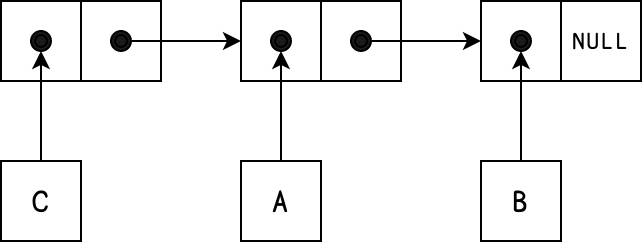
\includegraphics[width=0.4\textwidth]{figures/plist_2.png}
\caption{A list with atom C prepended}
\end{figure}

\par All pointers to the existing data are still valid and point to the same list as before. Appending to a list requires copying it, since the \textit{NULL} tail is being replaced to the pointer with the appended node, meaning that every pointer to the list points to the modified list now, which is undesirable.

\begin{figure}[H]
\centering
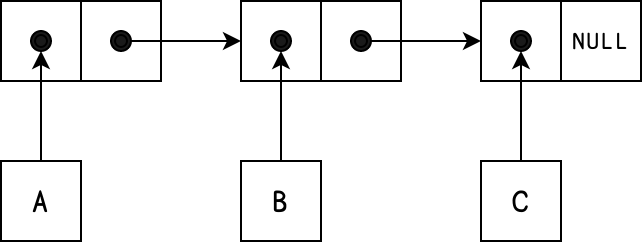
\includegraphics[width=0.4\textwidth]{figures/plist_4.png}
\caption{A list with atom C appended}
\end{figure}

\par List cloning in this case isn't deep. Considering the following deep list:

\begin{figure}[H]
\centering
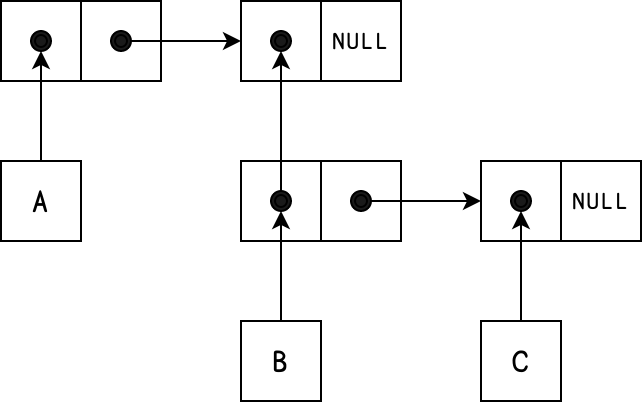
\includegraphics[width=0.4\textwidth]{figures/plist_6.png}
\caption{A list consisting of atom A and a list containing atoms B and C}
\end{figure}

\par Appending to this list involves changing the node at the end of it. As the atoms inside of it are unaffected (including nested lists), a deep clone isn't performed, since it isn't needed\footnote{MalbolgeLISP doesn't perform deep clones under any circumstances}:

\begin{figure}[H]
\centering
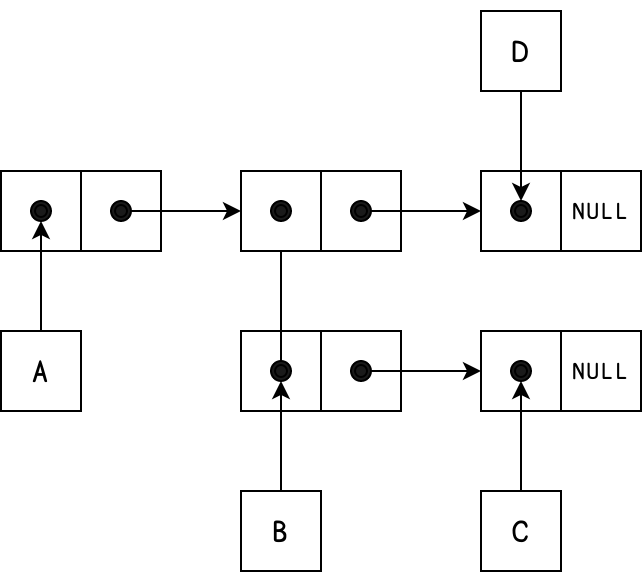
\includegraphics[width=0.4\textwidth]{figures/plist_5.png}
\caption{A list consisting of atom A and a list containing atoms B and C}
\end{figure}

\par Consequently, \verb|cons| will always be faster than \verb|append| or \verb|append'| (for merging lists, \verb|append'| will always be faster than a loop invoking \verb|append| repeatedly, since it doesn't perform nearly as many linked list pointer indirections - $O(m + n)$ compared to $O(m(m+1)/2+n) \Leftrightarrow O(m^2 + n)$).

\par An interesting special case of list cloning is related to the higher order functions related to point-free programming. Namely, when evaluated, \verb|selfie|, \verb|commute|, \verb|lazy|, \verb|fork|, partially applied functions, and reverse partial applications will clone their code lists. This happens since the code lists are sometimes evaluated, changed and evaluated again many times (\verb|map|'s behavior), and the data perceived by lazily evaluated values might change in an undesirable way - for instance, \verb|((atop #1 map) (bind lazy ~) '(0 1 1 1 1 0))| could yield \verb|1|, while \verb|0| was expected.


\section{The error table}

\par The following table lists all of the possible error messages that may be displayed by MalbolgeLISP during the evaluation of a given LISP expression:

\begin{longtable}{ | p{6em} | p{34em} | }
\hline
\textbf{Error code} & \textbf{Description}                                                                                                                           \\ \hline
\verb|E000|          & Invalid amount of arguments passed to \verb|if|.                                                                                               \\ \hline
\verb|E001|          & Invalid amount of arguments passed to \verb|quote| (usually used as \verb|'|).                                                                 \\ \hline
\verb|E002|          & Invalid amount of arguments passed to \verb|def|, or the first argument isn't a string atom.                                                   \\ \hline
\verb|E003|          & Invalid amount of arguments passed to \verb|lambda|, or the first argument isn't a list.                                                       \\ \hline
\verb|E004|          & Invalid amount of arguments passed to \verb|defun|, or the first argument isn't a string atom, or the second argument isn't a list.            \\ \hline
\verb|E005|          & Invalid amount of arguments passed to \verb|defmacro|, or the first argument isn't a string atom, or the second argument isn't a list.         \\ \hline
\verb|E006|          & \verb|bind| and \verb|bind'| require at least two additional arguments - the function to bind to, and at least one argument to apply.          \\ \hline
\verb|E007|          & \verb|atop| requires at least two additional arguments - at least two functions are required for composition.                                  \\ \hline
\verb|E008|          & \verb|monad| and \verb|dyad| require only one additional argument - the code block in which \verb|x| or \verb|x| and \verb|y| should be bound. \\ \hline
\verb|E009|          & Invalid amount of arguments passed to an user-defined closure or function.                                                                     \\ \hline
\verb|E010|          & The arithmetic operations require exactly two additional arguments.                                                                            \\ \hline
\verb|E011|          & The arithmetic operations can work only on numbers, but an atom of different type was supplied.                                                \\ \hline
\verb|E012|          & Invalid amount of arguments passed to \verb|=| - only two atoms can be compared. Use \verb|uniq| and \verb|size| to check the equality of more atoms at a time. \\ \hline
\verb|E013|          & Invalid amount of arguments passed to \verb|/=| - only two atoms can be compared.                                                              \\ \hline
\verb|E014|          & Invalid amount of arguments passed to \verb|~|.                                                                                                \\ \hline
\verb|E015|          & The only argument passed to \verb|~| isn't numeric.                                                                                            \\ \hline
\verb|E016|          & Invalid amount of arguments passed to \verb|!|.                                                                                                \\ \hline
\verb|E017|          & The only argument passed to \verb|!| isn't numeric.                                                                                            \\ \hline
\verb|E018|          & Invalid amount of arguments passed to \verb|+'| or \verb|-'|.                                                                                  \\ \hline
\verb|E019|          & The arguments passed to \verb|+'| or \verb|-'| aren't numeric.                                                                                 \\ \hline
\verb|E020|          & Invalid invocation of \verb|car| or \verb|cdr| (expected a single extra list argument)                                                         \\ \hline
\verb|E021|          & Invalid amount of arguments passed to \verb|cons|.                                                                                             \\ \hline
\verb|E022|          & Invalid right argument passed to \verb|cons| (expected a list, pairs are unsupported).                                                         \\ \hline
\verb|E023|          & Invalid amount of arguments passed to \verb|atom|.                                                                                             \\ \hline
\verb|E024|          & Invalid amount of arguments passed to \verb|print|.                                                                                            \\ \hline
\verb|E025|          & Invalid type of argument passed to \verb|cond| (expects lists).                                                                                \\ \hline
\verb|E026|          & Non-exhaustive \verb|cond|.                                                                                                                    \\ \hline
\verb|E027|          & Invalid invocation of \verb|let| (expected two lists).                                                                                         \\ \hline
\verb|E028|          & No \verb|let| bindings or an unbalanced binding exists.                                                                                        \\ \hline
\verb|E029|          & Invalid amount of arguments passed to \verb|iota|.                                                                                             \\ \hline
\verb|E030|          & Invalid type of argument passed to \verb|iota| (expected number).                                                                              \\ \hline
\verb|E031|          & Invalid amount of arguments passed to \verb|size|.                                                                                             \\ \hline
\verb|E032|          & The only argument passed to \verb|size| isn't a list.                                                                                          \\ \hline
\verb|E034|          & Invalid amount of arguments passed to \verb|nth|.                                                                                              \\ \hline
\verb|E035|          & Invalid argument types passed to \verb|nth| (expected a number and a list).                                                                    \\ \hline
\verb|E036|          & Out of bounds access using \verb|nth|, \verb|#N| or \verb|$N|.                                                                                 \\ \hline
\verb|E037|          & Invalid amount of arguments passed to \verb|flatmap| or \verb|map|.                                                                            \\ \hline
\verb|E038|          & Invalid type of 2nd argument passed to \verb|flatmap| or \verb|map| (expected a list).                                                         \\ \hline
\verb|E039|          & Invalid amount of arguments passed to \verb|filter|.                                                                                           \\ \hline
\verb|E040|          & Invalid type of 2nd argument passed to \verb|filter| (expected a list).                                                                        \\ \hline
\verb|E041|          & \verb|filter|'s functor returned an invalid type.                                                                                              \\ \hline
\verb|E042|          & Invalid amount of arguments passed to \verb|eval|.                                                                                             \\ \hline
\verb|E043|          & Invalid amount of arguments passed to \verb|append|.                                                                                           \\ \hline
\verb|E044|          & Invalid amount of arguments passed to \verb|append'|.                                                                                          \\ \hline
\verb|E045|          & Invalid type of arguments passed to \verb|append'| (expected a non-null list as the first argument and a list as the second argument).         \\ \hline
\verb|E046|          & Invalid type of argument passed to the monadic overload of \verb|rev|.                                                                         \\ \hline
\verb|E047|          & Invalid type of arguments passed to the dyadic overload of \verb|rev| (expected a number $N$ and a list $L$, where \verb|[(size L) > N]|).     \\ \hline
\verb|E048|          & Unrecognised overload of \verb|rev|.                                                                                                           \\ \hline
\verb|E049|          & Invalid amount of arguments passed to \verb|any| or \verb|every|.                                                                              \\ \hline
\verb|E050|          & The second argument passed to \verb|any| or \verb|every| isn't a list.                                                                         \\ \hline
\verb|E051|          & \verb|any|'s or \verb|every|'s functor returned an invalid type.                                                                               \\ \hline
\verb|E052|          & Invalid type of argument passed to the monadic overload of \verb|sort|.                                                                        \\ \hline
\verb|E053|          & Invalid type of element in a list passed to the monadic overload of \verb|sort| (monadic \verb|sort| can sort only numbers, due to lack of total ordering on other atoms). \\ \hline
\verb|E054|          & Invalid type of 2nd argument passed to the dyadic overload of \verb|sort|.                                                                     \\ \hline
\verb|E055|          & \verb|sort|'s functor returned an invalid type.                                                                                                \\ \hline
\verb|E056|          & Unrecognised overload of \verb|sort|.                                                                                                          \\ \hline
\verb|E057|          & Invalid amount of arguments passed to \verb|zip|.                                                                                              \\ \hline
\verb|E058|          & Invalid type of arguments passed to \verb|zip| (expected two lists).                                                                           \\ \hline
\verb|E059|          & Invalid amount of arguments passed to \verb|id|.                                                                                               \\ \hline
\verb|E060|          & Invalid amount of arguments passed to \verb|flatten|.                                                                                          \\ \hline
\verb|E061|          & Invalid type of argument passed to \verb|flatten| (expected a list).                                                                           \\ \hline
\verb|E062|          & Invalid amount of arguments passed to \verb|tie| (expected at least two arguments; to create a single element list use \verb|cons|).           \\ \hline
\verb|E063|          & Invalid amount of arguments passed to \verb|where|.                                                                                            \\ \hline
\verb|E064|          & Invalid type of argument passed to \verb|where| (expected a list).                                                                             \\ \hline
\verb|E065|          & Invalid type of element in a list passed to \verb|where| (expected a number).                                                                  \\ \hline
\verb|E066|          & Invalid amount of arguments passed to \verb|iterateN| (expected at least three arguments).                                                     \\ \hline
\verb|E067|          & Invalid type of amount of iterations specified in an invocation to \verb|iterateN| (expected a number).                                        \\ \hline
\verb|E068|          & Invalid amount of arguments passed to \verb|iterate| (expected at least three arguments).                                                      \\ \hline
\verb|E069|          & \verb|iterate|'s functor returned an invalid type (expected boolean).                                                                          \\ \hline
\verb|E070|          & Invalid amount of arguments passed to \verb|fold| or \verb|fold'| (expected two arguments for \verb|fold'|, or three for \verb|fold| - the identity element). \\ \hline
\verb|E071|          & Invalid type of the last argument passed to \verb|fold| or \verb|fold'| (expected a list).                                                     \\ \hline
\verb|E072|          & Invalid amount of arguments passed to \verb|zipwith| (expected three arguments).                                                               \\ \hline
\verb|E073|          & Last two arguments passed to \verb|zipwith| aren't lists.                                                                                      \\ \hline
\verb|E074|          & Invalid amount of arguments passed to \verb|replicate| (expected two arguments).                                                               \\ \hline
\verb|E075|          & The dyadic \verb|list list| overload to \verb|replicate| expects only numbers in the first list.                                               \\ \hline
\verb|E076|, \verb|E077| & Invalid argument types passed to \verb|replicate| (expected \verb|list list|, \verb|number list|, or \verb|number number|).                 \\ \hline
\verb|E078|          & Invalid amount of arguments passed to \verb|count| (expected two arguments).                                                                   \\ \hline
\verb|E079|          & The second argument passed to \verb|count| was expected to be a list.                                                                          \\ \hline
\verb|E080|          & \verb|count|'s functor returned an invalid type.                                                                                               \\ \hline
\verb|E081|          & Invalid amount of arguments passed to \verb|take| or \verb|drop'| (expected two arguments).                                                    \\ \hline
\verb|E082|          & Invalid type of arguments passed to \verb|take| or \verb|drop'| (expected \verb|number list|).                                                 \\ \hline
\verb|E083|          & Invalid amount of arguments passed to \verb|drop| or \verb|take'| (expected two arguments).                                                    \\ \hline
\verb|E084|          & Invalid type of arguments passed to \verb|drop| or \verb|take'| (expected \verb|number list|).                                                 \\ \hline
\verb|E085|          & Invalid amount of arguments passed to \verb|intersperse| (expected two arguments).                                                             \\ \hline
\verb|E086|          & The second argument passed to \verb|intersperse| was expected to be a list.                                                                    \\ \hline
\verb|E087|          & Invalid amount of arguments passed to \verb|scan| or \verb|scan'| (expected two arguments for \verb|scan'|, or three for \verb|scan| - the identity element). \\ \hline
\verb|E088|          & Invalid type of the last argument passed to \verb|scan| or \verb|scan'| (expected a list).                                                     \\ \hline
\verb|E089|          & Invalid amount of arguments passed to \verb|selfie| (expected two arguments).                                                                  \\ \hline
\verb|E090|          & Invalid amount of arguments passed to \verb|commute| (expected three arguments).                                                               \\ \hline
\verb|E091|          & Invalid amount of arguments passed to \verb|uniq| (expected a single argument).                                                                \\ \hline
\verb|E092|          & Invalid argument type passed to \verb|uniq| (expected a list).                                                                                 \\ \hline
\verb|E093|          & Unrecognised built-in function.                                                                                                                \\ \hline
\verb|E094|          & Invalid user-defined macro invocation (invalid amount of arguments supplied).                                                                  \\ \hline
\verb|E095|          & Can't evaluate (attempted to evaluate a numeric list without quoting?)                                                                         \\ \hline
\verb|E096|          & Invalid amount of arguments passed to \verb|fork| (expected at least two arguments).                                                           \\ \hline
\verb|E097|          & Invalid amount of arguments passed to constant n-th (expected a single argument).                                                              \\ \hline
\verb|E098|          & Invalid type of argument passed to constant n-th (expected a list).                                                                            \\ \hline
\verb|E099|          & Invalid amount of arguments passed to \verb|lazy| (expected at least two arguments).                                                           \\ \hline
\verb|E100|          & Invalid amount of arguments passed to \verb|lift| (expected two arguments).                                                                    \\ \hline
\verb|E101|          & Invalid type of second argument passed to \verb|lift| (expected a list).                                                                       \\ \hline
\verb|E102|          & Invalid amount of arguments passed to \verb|bruijn| (expected a single argument).                                                              \\ \hline
\verb|E103|          & Invalid type of the argument passed to \verb|bruijn| (expected a number).                                                                      \\ \hline
\verb|E104|          & Not enough lambda expressions in scope for \verb|bruijn| invocation.                                                                           \\ \hline
\end{longtable}


\section{Value types}

\par MalbolgeLISP supports many built-in value types. The logical types (as recognised by the built-in functions) differ from the types actually implemented in the interpreter.

\par The boolean type in MalbolgeLISP doesn't exist. Instead, the numerical value \verb|0| is considered falsy, and every other value is considered truthy. Built-in functions will always return either \verb|0| or \verb|1| to represent a boolean value.

\par The built-in higher order functions don't have the notion of a callable type. For example, \verb|+| (outside of being an unbound atom which happens to be recognised as a built-in function) is a valid callable type, just like the result of binding, atops, forks, macros, lazily evaluated values and lambda expressions. Since they all are considered (internally) callable types, but most of them don't have a canonical representation (like lambda expressions do), they are considered \textit{synthetic} types. When printed, the interpreter will use \verb|bind/syn|, \verb|macro/syn| or \verb|lazy/syn| to represent them.

\par There isn't a separate type for quoted values. Instead, quoting simply prevents evaluation (since the \verb|'(...)| syntactic sugar is translated into \verb|(quote (...))|, and \verb|quote| is a built-in function that returns it's argument without evaluating it).

\par MalbolgeLISP doesn't support pairs. For this reason, \verb|cons| always assumes its right argument is a list (or \textit{null}). \verb|tie|\footnote{In other implementations also called \verb|list| -  \url{https://www.cs.cmu.edu/Groups/AI/html/cltl/clm/node149.html}} is a more convenient version of \verb|cons|, since \verb|(tie a b c ... z)| is always equivalent to a ladder of invocations to \verb|cons| - \verb|(cons a (cons b (cons c ... (cons z null))))|. Lists can also be untied (a callable object is evaluated so that an arbitrary list is treated as the parameter list). The following function accomplishes this using continued partial application:

\begin{minted}{lisp}
(defun untie (f args) (
    (if (= null args)
        (f)
        (untie (bind f (car args)) (cdr args))))
\end{minted}

\par A more efficient version of this function could be made using \verb|iterate| or \verb|iterateN|, but instead of using a Lisp implementation of \verb|untie|, the built-in \verb|lift| function can be used (accomplishing the same result more efficiently).

\section{Lambda expressions, functions and macros}

\par In MalbolgeLISP code, lambda expressions are ubiquitous as a form of binding variables (\verb|let| uses a lambda expression in it's implementation), defining recursive functions (since point-free programming is generally considered to not be able to represent recursion, but it might be possible for some special, simple cases using \verb|iterate| and \verb|iterateN|\footnote{\url{https://dfns.dyalog.com/n_tacit.htm}}), or functions too complex to be represented entirely in point-free style. Sometimes they are also preferred to point-free expressions, since programmers find them harder to read\footnote{\url{https://spin.atomicobject.com/2017/09/29/point-free-notation/}}.

\par Lambda expressions in MalbolgeLISP v1.2 follow the rules of lexical (static) scoping, meaning that the lexical ancestor's bound variables are visible inside the lambda expression, but they also can be shadowed using \verb|let| bindings or \verb|lambda| arguments. MalbolgeLISP v1.0 didn't have the concept of scoping, and a few public pre-release versions of MalbolgeLISP v1.1 employed dynamic scoping, meaning that the caller's bound variables are visible inside the lambda expression.

\par The \verb|defun| built-in function is defined as syntactic sugar over \verb|def| and \verb|lambda|, so that \verb|(defun a (x y z ...) (...)| is equivalent to \verb|(def a (lambda (x y z ...) (...)))|. Functions can also be defined without the lambda expression overhead\footnote{caused \textit{inter alia} by lexical scoping} as tacit expressions. Monadic and dyadic functions can be defined using \verb|monad| and \verb|dyad| built-in functions, which are syntactic sugar over \verb|(lambda (x) (...))| and \verb|(lambda (x y) (...))| respectively.

\par In MalbolgeLISP, a macro is considered to be equivalent to a function, except it doesn't have the concept of scoping, and macro arguments aren't evaluated\footnote{meaning that variables aren't expanded, lists don't need quoting, etc...}. Since the main inefficiencies of lambda expressions don't apply to macros, they tend to be much more efficient. Macro representation also more efficient, since macros are stored as a single list of arguments and the code, without the auxiliary structure and pointer indirection to the code and cloned symbol table (as observed in lambda expressions).

\section{Point-free programming}

\par Point-free programming (also called tacit programming) is one of MalbolgeLISP's strong sides. It's facilitated using a wide range of advanced primitive functions\footnote{tacks, constant \verb|n-th|, \verb|tie|, \verb|atop|s, monad lifting - \verb|fork|s, \verb|bind|s and reverse binds}. Tacit programming is all about transformations on functions and their data, so that the computation can be expressed without explicitly naming the parameters and creating direct functions. MalbolgeLISP implements or faciliates the following functions and concepts:

\begin{itemize}
    \item The monadic identity function \verb|id|, for which \verb|id x| $\Leftrightarrow$ \verb|x| holds. Equivalent to \verb|$0|.
    \item A partial application higher order function \verb|bind|, for which \verb|(bind f x y...) a b...| $\Leftrightarrow$ \verb|f x y... a b...| holds.
    \item A reverse partial application higher order function \verb|bind'|, for which the identity \verb|(bind' f x y...) a b...| $\Leftrightarrow$ \verb|f a b... x y...| holds.
    \item The variadic identity function (a \textit{tack}\footnote{\url{https://aplwiki.com/wiki/Identity}}) - a $\mu$-recursive primitive projection function ${\displaystyle P_{i}^{k}(x_{1},\ldots ,x_{k}){\stackrel {\mathrm {def} }{=}}x_{i}\,}$ with implied $k$.
    \item The $\mu$-recursive primitive constant function \verb|bind $0 n|, defined as ${\displaystyle C_{n}^{k}(x_{1},\ldots ,x_{k}){\stackrel {\mathrm {def} }{=}}n}$.
    \item Variadic monad lifting function \verb|fork| (the $\mu$-recursive substitution operator). Given an $m$-ary function $h(x_{1},\ldots ,x_{m})\,$ - \textit{reductor}, and $m$ $k$-ary functions $g_{1}(x_{1},\ldots ,x_{k}),\ldots ,g_{m}(x_{1},\ldots ,x_{k})$ - \textit{reductees}, it is known that $h \circ (g_{1},\ldots ,g_{m}){\stackrel {\mathrm {def} }{=}}f $ where $ f(x_{1},\ldots ,x_{k})=h(g_{1}(x_{1},\ldots ,x_{k}),\ldots ,g_{m}(x_{1},\ldots ,x_{k}))$ holds.
    \item A variation of primitive $\mu$-recursive recursion operator \verb|iterateN|\footnote{\url{http://help.dyalog.com/15.0/Content/Language/Primitive\%20Operators/Power\%20Operator.htm}}. Given the $k$-ary function $g(x_{1},\ldots ,x_{k})\,$ the iteration count $n$ and $k$ parameters $r_1$ up to $r_k$: \[
        \rho (g,n,r_1,...,r_k){\stackrel {\mathrm {def} }{=}}
          \begin{cases}
            g(\rho(g, n-1, r_1,\ldots , r_k), r_2,\ldots , x_k), & \text{for } n > 1 \wedge k \ge 2 \\
            g(\rho(g, n-1, r_1)), & \text{for } n > 1 \wedge k = 1 \\
            g(r_1,\ldots , r_k), & \text{for } n = 1 \wedge k \ge 2 \\
            g(r_1), & \text{for } n = 1 \wedge k = 1 \\
            r_1, & \text{for } n = 0
          \end{cases}
    \]
    \item A variation of the \verb|iterateN| higher order function, which decides if the function will be iterated further based on the previous and current result. For instance, \verb|bind iterate =| is a limit operator (applying a function until the result is stable).
    \item A varaidic function composition operator \verb|atop|, for which \verb|(atop f g h...) x y...| $\Leftrightarrow$ \verb|f (g (h... x y))| holds.
    \item \verb|tie|, \verb|lift|, and constant \verb|n-th| functions for handling variadicity using lists.
    \item A concept derived from De Bruijn indices, \verb|bruijn N| yielding the $n$-th lambda expression in scope, assuming $0$ is the current one, $1$ is it's lexical ancestor, etc...
\end{itemize}

One can build further on the mentioned concepts to introduce point-free programming idioms:

\begin{itemize}
    \item Due to the variadic nature of \verb|fork|, if it's invocation involves multiple functions, the resulting list sometimes can't be applied to many functions. For this reason, the idiom consisting of \verb|tie| and \verb|atop| is used to turn all the results into a list, to then use it with a function (which is often a \verb|fold|) - \verb|fork (atop f tie) g h|.
    \item In \verb|fork|s, \textit{tacks} are often used as reductees to copy a specified argument to the reductor. For instance, the following APL-style tacit inner product function utilises this idiom: \begin{verbatim}
; MalbolgeLISP
% (def . (fork fold' $0 (fork zipwith $1 $2 $3)))
...................|........................
(fold' $0 (zipwith $1 $2 $3))
% [+ . * '(1 2 3) '(4 5 6)]
....................|........................................
32

⍝ APL
      1 2 3 +.× 4 5 6
32
    \end{verbatim}
    \item In tacit expressions, square bracket lists (denoted by \verb|[]|) are often used, since they allow separation of \verb|fork|'s reductor from it's reductees, improving the readability (as an alternative to \verb|{}| syntax). They are also used alongside \verb|bind| and \verb|bind'|. For example, a defined average function could be translated in the following way:
    \begin{verbatim}
; Average of list x is the sum of it divided by it's size. Assumes size >= 1.
(def avg (monad [[+ fold' x] / (size x)]))
(def avg (monad ([/ fork [fold' bind +] size] x)))
(def avg [/ fork [fold' bind +] size])
; Using the dedicated fork syntax.
(def avg {/ [fold' bind +] size})
    \end{verbatim}
    \item Tack factoring is used to optimise certain fork expressions - \verb|(fork f (atop g $0) (atop h $0))| $\Leftrightarrow$ \verb|(atop (fork f g h) $0)|. Tack factoring also works for tack reductees, since \verb|$0| is equivalent to \verb|(atop id $0)|.
    \item Commuting sometimes allows to avoid forks - \verb|{f $1 $0}| $\Leftrightarrow$ \verb|(bind commute f)|. Although, since most tacit expressions tend to involve \verb|bind|, \verb|bind'| can be used instead of \verb|commute|: \verb|{+ (bind' / 2) 32}| is more efficient than \verb|{+ (bind commute / 2) 32}|.
    \item Duplicating arguments - \verb|{f $0 $0}| $\Leftrightarrow$ \verb|(bind selfie f)|.
    \item Lifting lists - \verb|(lift f '(x y z...))|\footnote{the list doesn't have to be specified inline} $\Leftrightarrow$ \verb|f x y z...|.
\end{itemize}

\par \verb|commute| and \verb|selfie| can be re-implemented in Lisp as follows:
\begin{minted}{lisp}
(def selfie' (dyad (x y y)))
(defun commute' (x y z) (x z y))
\end{minted}

\par Since MalbolgeLISP offers first class functions, lazy evaluation, short-circuiting inside tacit expression, arbitrary forks, atops and arbitrary tacks, MalbolgeLISP's tacit programming model is superior to APL's\footnote{\url{https://dfns.dyalog.com/n_tacit.htm}}, making many concepts much easier to express.

\section{Numerical algorithms}

\par MalbolgeLISP implements a set of basic numerical algorithms - greatest common divisor, least common multiple, power and factorial.

\par The factorial function's value grows very quickly, so it can be pre-computed using a lookup table, meaning that factorials can be yielded without expensive computation. The following APL program has been used to generate the lookup table:

\begin{verbatim}
{∊'{'(','(1↓∘,,⍤0)⍕¨m/⍨⍵≥m←!⍳20)'}'}2*26
\end{verbatim}

\par The MalbolgeLISP code guards against out of bounds accesses by returning 0 on overflow:

\begin{verbatim}
&f_table
$(gen_vec({1,2,6,24,120,720,5040,40320,362880,3628800,39916800}))

@fact
    cle r2, 11
    clr r1
    cmov r1, *f_table
    cadd r1, r2
    crcl r1, r1
    ret
\end{verbatim}

\par The power function implementation utilises the binary exponentiation algorithm to achieve better performance. The recursive implementation used in past versions of MalbolgeLISP follows:

\begin{verbatim}
@pow
    ceq r3, 0
    cmov r1, 1
    cret
    push r3
    asr r3
#call("pow")
    pop r3
    ; XXX: for brainfuck target, use a diff. encoding
    mul r1, r1
    mod r3, 2
    cne r3, 0
    cmul r1, r2
    ret
\end{verbatim}

\par MalbolgeLISP v1.2 employs the improved, iterative version of the algorithm:

\begin{verbatim}
@pow
    mov r1, 1
@pow_loop
    ceq r3, 0
    cret
    mov r4, r3
    mod r4, 2
    ceq r4, 1
    cmul r1, r2
    ; XXX: use diff. encoding for bf target
    mov r4, r2
    mul r2, r4
    asr r3
    jmp %pow_loop
\end{verbatim}

\par Greatest common divisor is implemented using an algorithm utilising two Euclidean division operations\footnote{which proves itself to be faster than the standard Euclidean algorithm, due to the Malbolge toolchain intricacies} and the least common multiple function is defined using the following formula:

\[
    \text{lcm}(a, b) = \frac{ab}{\text{gcd}(a, b)}
\]

\begin{verbatim}
@gcd
    ceq r2, 0
    cret
    mod r1, r2
    cne r1, 0
    cmod r2, r1
    cjnz %gcd
    mov r1, r2
    ret

@lcm
    mov r3, r1
    mul r3, r2
#call("gcd")
    div r3, r1
    mov r1, r3
    ret
\end{verbatim}

\section{Laziness and side effects}

\par MalbolgeLISP provides first-class support for lazy evaluation. Lazily evaluated expressions are introduced to the code using the \verb|lazy| built-in word or, alternatively, the \verb|?| list prefix. Laziness is implemented similarly to how Java\footnote{via the \verb|Supplier<T>| (\url{https://docs.oracle.com/javase/8/docs/api/java/util/function/Supplier.html}) class and wrapping the computation in a lambda expression} or C++\footnote{via suspected function; explained in more detail in Appendix B - although some more sophisticated attempts were made: \url{https://github.com/MarcDirven/cpp-lazy}.} achieve it. Speaking from a high-level point of view, the computation is wrapped in a closure, and when the value is requested, the closure is evaluated and the result takes place of the lazily evaluated atom\footnote{this technique is called \textit{memoization}}. The concepts of memoization and lazy evaluation are illustrated on the following example:

\begin{Verbatim}[commandchars=\\\{\}]
\textcolor{Maroon}{; Define a product function that has a side effect of printing,}
\textcolor{Maroon}{; so that it's known when the value is evaluated and memoized.}
\textcolor{BlueViolet}{% (defun yelling_prod (x y) (lazy print [x * y]))}
.....................|.
(lambda (x y) (lazy print (* x y)))
\textcolor{Maroon}{; Define an eager product function.}
\textcolor{BlueViolet}{% (defun eager_prod (x y) (print [x * y]))}
....................|.
(lambda (x y) (print (* x y)))
\textcolor{Maroon}{; The lazy version took less steps to evaluate, since the}
\textcolor{Maroon}{; product wasn't computed. the lazy version also didn't}
\textcolor{Maroon}{; print anything, unlike the eager version.}
\textcolor{BlueViolet}{% (def l1 (yelling_prod 9 9))}
...........|.......
lazy/syn
\textcolor{BlueViolet}{% (def e1 (eager_prod 9 9))}
...........|...........
81

81
\textcolor{Maroon}{; Since the value of the lazy version is required to produce}
\textcolor{Maroon}{; a result, it's evaluated (because 81 is printed).}
\textcolor{Maroon}{; The evaluation was deferred.}
\textcolor{BlueViolet}{% (print [e1 + [l1 + ?(+ 2 2)]])}
.....................|..............
81
......
166

166
\textcolor{Maroon}{; Because the value of l1 was memoized, the evaluation of l1}
\textcolor{Maroon}{; is instant.}
\textcolor{BlueViolet}{% e1}
.|.
81
\textcolor{BlueViolet}{% l1}
.|.
81
\end{Verbatim}

\par Lazy evaluation can reduce the run-time of more complex algorithms\footnote{assuming one ignores the overhead of lazily evaluated values, which can sometimes make the difference too subtle or worsen the matters} - if \verb|lazy| is omitted in the expression \verb|((atop #1 map) (bind lazy selfie *) (iota 9))|, it takes 5 more seconds to evaluate (since the \verb|map| functor is being applied eagerly over each of the indices, and conclusively, only the second element from the list is desired). The difference would be even more noticeable if the \verb|map| functor was an expensive operation.

\par Since lazy evaluation makes the side effect handling difficult at times, an equivalent of the Haskell's IO monad could be beneficial to MalbolgeLISP, although the only side effect MalbolgeLISP supports is evaluated output (via \verb|print|). Input isn't supported, because it's mutually exclusive with existence of the evaluation progress bar. For this reason, no way to sequence operations comparable to Haskell's IO monad or \verb|do| blocks is supported in MalbolgeLISP.

\section{Missing features}

\par MalbolgeLISP is missing a few features that are generally considered convenient\footnote{sometimes even essential, although they can be synthesised in MalbolgeLISP using macros}. The following list provides a rationale behind every missing feature:

\begin{itemize}
    \item \textbf{Negative numbers} - they would require special handling in multiplication and division routines, special handling in integer printing routines and comparison routines, causing a huge performance overhead for little to no gain.
    \item \textbf{String constants} - MalbolgeLISP has no \textit{actual} strings, only unbounded atoms. Because the author's vision of string handling in MalbolgeLISP would involve orthogonal operations for ordinary lists and strings (\textit{lists of characters}), string syntax would be implemented as syntactic sugar over lists.
    \item \textbf{Floating point arithmetic}, \textbf{fixed point arithmetic}, \textbf{fractional arithmetic} - floating point arithmetic would make the codebase too complex (as in the signed integer case) for very little gain, since floating point arithmetic could be replaced by the more efficient fixed point arithmetic or fractional arithmetic. Fixed point arithmetic wasn't implemented in primitives, since it would lead to breaking the orthogonality of arithmetic functions. Fractional arithmetic wasn't implemented, since it can be easily introduced to MalbolgeLISP as a set of functions, without taxing the interpreter's size.
    \item \textbf{Pairs} - the support for them would complicate the interpreter code for no reason. They can be implemented as macros or functions with little overhead, since representing pairs as lists isn't remarkably inefficient.
    \item \textbf{Garbage collection or reference counting} - a lot of the MalbolgeLISP codebase depends on the properties of a bump allocator\footnote{freshly allocated memory is zeroed, references to old objects persist, so they may be reused at some point}. Precise reference counting in MalbolgeLISP would cause too much overhead and would be difficult to implement because of the limitations in tooling. Garbage collection suffers from the same issues, but much more exaggerated - a garbage collector would require scanning the stack and walking the entire memory, then compacting it, adjusting all the pointers and tweaking the internal bump allocator pointer. Since this garbage collector design is conservative, it's not guaranteed to be precise. Different garbage collection algorithms would require a more intricate design and resources.
\end{itemize}
